% --- Template for thesis / report with tktltiki2 class ---
% 
% last updated 2013/02/15 for tkltiki2 v1.02

\documentclass[finnish]{tktltiki2}

% tktltiki2 automatically loads babel, so you can simply
% give the language parameter (e.g. finnish, swedish, english, british) as
% a parameter for the class: \documentclass[finnish]{tktltiki2}.
% The information on title and abstract is generated automatically depending on
% the language, see below if you need to change any of these manually.
% 
% Class options:
% - grading                 -- Print labels for grading information on the front page.
% - disablelastpagecounter  -- Disables the automatic generation of page number information
%                              in the abstract. See also \numberofpagesinformation{} command below.
%
% The class also respects the following options of article class:
%   10pt, 11pt, 12pt, final, draft, oneside, twoside,
%   openright, openany, onecolumn, twocolumn, leqno, fleqn
%
% The default font size is 11pt. The paper size used is A4, other sizes are not supported.
%
% rubber: module pdftex

% --- General packages ---

\usepackage[utf8]{inputenc}
\usepackage[T1]{fontenc}
\usepackage{lmodern}
\usepackage{microtype}
\usepackage{amsfonts,amsmath,amssymb,amsthm,booktabs,color,enumitem,graphicx}
\usepackage[pdftex,hidelinks]{hyperref}
\graphicspath{ {images/} }
% Automatically set the PDF metadata fields
\makeatletter
\AtBeginDocument{\hypersetup{pdftitle = {\@title}, pdfauthor = {\@author}}}
\makeatother

% --- Language-related settings ---
%
% these should be modified according to your language

% babelbib for non-english bibliography using bibtex
\usepackage[fixlanguage]{babelbib}
\selectbiblanguage{finnish}

% add bibliography to the table of contents
\usepackage[nottoc]{tocbibind}
% tocbibind renames the bibliography, use the following to change it back
\settocbibname{Lähteet}

% --- Theorem environment definitions ---

\newtheorem{lau}{Lause}
\newtheorem{lem}[lau]{Lemma}
\newtheorem{kor}[lau]{Korollaari}

\theoremstyle{definition}
\newtheorem{maar}[lau]{Määritelmä}
\newtheorem{ong}{Ongelma}
\newtheorem{alg}[lau]{Algoritmi}
\newtheorem{esim}[lau]{Esimerkki}

\theoremstyle{remark}
\newtheorem*{huom}{Huomautus}


% --- tktltiki2 options ---
%
% The following commands define the information used to generate title and
% abstract pages. The following entries should be always specified:

\title{Reunalaskenta arkkitehtuurit}
\author{Lauri Vene}
\date{\today}
\level{Pro gradu -tutkielma}
\abstract{Tiivistelmä.}

% The following can be used to specify keywords and classification of the paper:

\keywords{reuna, pilvi, tietojenkäsittelytiede}

% classification according to ACM Computing Classification System (http://www.acm.org/about/class/)
% This is probably mostly relevant for computer scientists
% uncomment the following; contents of \classification will be printed under the abstract with a title
% "ACM Computing Classification System (CCS):"
% \classification{}

% If the automatic page number counting is not working as desired in your case,
% uncomment the following to manually set the number of pages displayed in the abstract page:
%
% \numberofpagesinformation{16 sivua + 10 sivua liitteissä}
%
% If you are not a computer scientist, you will want to uncomment the following by hand and specify
% your department, faculty and subject by hand:
%
% \faculty{Matemaattis-luonnontieteellinen}
% \department{Tietojenkäsittelytieteen laitos}
% \subject{Tietojenkäsittelytiede}
%
% If you are not from the University of Helsinki, then you will most likely want to set these also:
%
% \university{Helsingin Yliopisto}
% \universitylong{HELSINGIN YLIOPISTO --- HELSINGFORS UNIVERSITET --- UNIVERSITY OF HELSINKI} % displayed on the top of the abstract page
% \city{Helsinki}
%


\begin{document}

% --- Front matter ---

\frontmatter      % roman page numbering for front matter

\maketitle        % title page
\makeabstract     % abstract page

\tableofcontents  % table of contents
\

% --- Main matter ---

\mainmatter       % clear page, start arabic page numbering

\section{Huomioita}
\begin{itemize}
\item reuna
\item reunasolmu
\end{itemize}

Tutkielmassa puhutaan mobiililaitteesta, mutta monet toiminnallisuudet ovat sovellettavissa kaikenlaisiin mobiileihin laitteisiin, esimerkiksi kannettaviin tai älykkäisiin ajoneuvoihin. 

Listan Mobile Computingin neljästä pääasiallisesta rajoitteesta.\\
\textit{Unpredictable variation in network quality, lowered trust and robustness of
mobile elements, limitations on local resources imposed by
weight and size constraints, and concern for battery power
consumption} [13]

[13]M. Satyanarayanan, "Fundamental Challenges in Mobile Computing," Proc.
15th ACM Symp. Principles of Dist. Comp., Philadelphia, PA, May, 1996



\section{Johdanto}

\section{Reunalaskennan perusteet}

\subsection{Motivaatio}
Reunalaskennan ideana on täydentää ja avustaa resurssiköyhiä asiakaslaitteita. Mobiililaitteisiin voitaisiin teoriassa lisätä enemmän resursseja, mutta ne tulisivat kannettavuuden ja käyttöajan kustannuksella. 
Avustamiseksi voidaan ajatella esimerkiksi tilanne, jossa akkuvirtaa säästääkseen, mobiililaite välittää resurssi intensiivisen laskutoimituksen reunasolmulle laskettavaksi. Reunasolmun voi ajatella kevennetyksi versioksi palvelimesta joten sen rajoitteet ovat hyvin erilaiset kuin asiakaslaitteen.
Täydentävä toiminta reunalaskennan avulla tarkoittaa asiakaslaitteen resurssin puutetta suoriutua jostakin tehtävästä. Esimerkiksi muistin riittämättömyys kuvankäsittelyyn. Tällöin voitaisiin esimerkiksi ottaa etäkäyttöyhteys reunasolmuun jolla käsittely tehdään. Asiakaslaitteelle jäisi tässä tilanteessa tehtäväksi ainoastaan esittää reunasolmun tilaa käyttäjälle.


Satyanarayana \cite{RefWorks:doc:5a65a2cee4b0cb152cfb50e7} esitti artikkelissaan pervasive computing esimerkkejä jokapaikan tietotekniikasta. Ympäristöön sijoitettujen laitteiden yhteistoiminnan avulla, asiakkaalle voidaan tarjota parempaa ja täsmällisempää palvelua. Yhtenä palvelun laadun ehtona on kyky ennakoida asiakkaan toimintaa.
Nykyään mobiililaitteilla on mahdollista hyödyntää langattomia yhteyksiä.
Suurin osa palvelinresursseista ja palveluiden tuottamiseen käytettävästä tiedosta  on keskittyneenä pilveen. Käytännössä minkä tahansa palvelun käyttäminen mobiililaitteella edellyttää yhteyttä näihin pilvipalveluihin. Pilvipalveluiden ylläpitäminen  

Toinen painopiste on siinä että tieto seuraa käyttäjää. Esimerkiksi pöytäkoneelta mobiililaitteeseen.(Satyanarayanan, 2001).
Cyber foraging, on termi jota käytetään kuvaamaan paradigmaa jossa laite etsii ympäristöstä hyödynnettävää tietoa ja avustajia/korvikkeita. Avustajan (surrogate) rooli on täydentää lähtökohtaisesti resurssirajallista laitetta, esimerkiksi suorittamalla laskentaa, jotta asiakaslaite voisi esimerkiksi säästää akkua.
Tähän toimintaan liittyy kuitenkin useita haasteita. Esimerkiksi kuinka asiakaslaite löytää avustajan? Mitäs jos avustaja on ruuhkautunut? Kuinka avustaja alustetaan ja kauanko siinä kestää? 
Nämä ovat keskeisiä kysymyksiä myös reunalaskennassa. 
Vastuun jakaminen asiakaslaitteen sekä reunanklusterin välillä on riippuvainen siitä, kuinka paljon avustusta asiakaslaite tarvitsee. 
Toiseen ääripäähän vietynä asiakaslaite on niin sanottu kevyt asiakaspääte (thin client), jolla ei olisi resursseja juurikaan mihinkään. Tällainen asiakaslaite joutuisi jakamaan kaiken laskennan eteenpäin avustajalle. 
Tämän kaltainen asiakaslaite olisi riippuvainen reunan mahdollisuuksista suorittaa palveluiden vaatimia toiminnallisuuksia. 
Seuraavana askeleena kohti itsenäisempää suoriutumista olisi asiakaslaite, joka pystyy osittain tarjoamaan käyttäjälle palveuita. Tämä laite tarvisi reunaklusterilta avustusta ainoastaan joissain tapauksissa. 
Viimeisenä toimijana olisi kokonaan itsenäinen asiakaslaite, joka tarvitsisi reunalta ainoastaan palveluita täydentäviä ominaisuuksia.
Tämä laite saattaisia turvautua reunalaskentaan esimerkiksi jos akku on vähissä, tai laitteella itsellään ei ole kaikea tarvittavaa tietoa laskennan suorittamiseksi.

\subsection{a}
\begin{itemize}
\item Mistä reunalaskenta koostuu? (Suurimmat toimijat, keskeisimmät toiminnot)
\item Mikä on MEC?
\item Reunalaskenta vai reunapalvelu?
\item MCC vai MEC?
\item Pilvi vai palvelinkeskus, palvelinresursseja.
\item Mitä reunalaskenta on?
\item Miksei siirretä laskentaa pilveen?
\item Mitkä ovat mobiilin ongelmat nykyisellään?
\item Mitkä ovat reunalaskennan haasteet?
\end{itemize}


Pilvipalvelulla tarkoitetaan palvelua, joka sijaitsee internetissä. Palvelut tarjotaan käyttäjälle verkkoyhteyden välityksellä.
Pilvipalvelut sisältävät usein suuria määriä laskenta- ja tallennusresursseja. Palvelut usein sijoitettu siten että ne ovat runkoverkossa kiinni, jolloin niiden voidaan ajatella sijaitsevan internetin "keskustassa".
Yleensä palveluita ylläpidetään keskitettyinä korkeintaan muutamaan eri konesaliin.
Pilvipalvelun palvelun kohde on usein asiakaslaite (UE, user equipment), joka sijaitsee internet-topologian näkökulmasta lehtisolmussa.

Reunalaskenta on yksi hajautetun laskennan muoto jossa 

Mobiililaitteiden yleisiä ominaisuuksia ovat resurssien vähyys ja akkuvirran rajallisuus. Mobiililaitteiden käyttö on myös usein riippuvaista langattomista verkkoyhteyksistä.
Palveluiden toiminta mobiililaitteilla on siis riippuvainen näiden kolmen ominaisuuden asettamista rajoista.
Laskentaresurssien lisääminen johtaisin lyhyempään käyttöaikaan akkuvirralla. Suurempi akku mahdollistaa pidemmän käyttöajan, mutta se tekisi laitteesta suuremman. Akun kokoa ja laskentaresurssien määrää pyritäänkin tasapainottamaan.
Voidaan pyrkiä minimoimaan laitteen virrankulutus esimerkiksi laittamalla laitteeseen heikkotehoisempi suoritin. Tämä näkyy siinä, millaisia palveluita mobiililaitteella voidaan tarjota.
Esimerkiksi kuvankäsittelyä tai muuta raskaampaa laskentaa vaativaa toiminnallisuutta ei voida tällaisella laitteella tehdä. 
Seuraava vaihtoehto olisi lähettää laskentaa tehokkaammille laitteille pilveen. Laskennan siirtäminen vie aikaa ja tällöin ei voida tarjota kovin reaaliaikaisia palveluita.
Siirrettyyn laskentaan kuluva aika koostuu pääasiassa verkon viiveestä, siirrosta ja itse laskennasta. 
Kokonaisuudessa siirtämiseen ja laskentaan kuluvan ajan määrään vaikuttaa pilven sijainti, verkon ruuhkaisuus, verkon kapasiteetti, sekä käytössä olevan laskentakapasiteetin määrä.
Reunalaskenta on konsepti, jonka avulla laskenta voidaan tuoda lähemmäksi käyttäjää.

Reunalaskennassa (MEC,Mobile Edge Computing vai MCC Mobile Cloud Computing?) on tarkoitus tuoda palvelinresursseja lähemmäksi käyttäjää. Reunalaskenta on osassa kirjallisuutta jaettu kahteen kategoriaan sen mukaan tarjotaanko palvelua RAN (Radio access network) vai yleisesti WAN yhteydessä. RAN verkossa toimivaa reunalaskentaa kutsutaan Multi-access edge computing ja muita reunalaskennan ratkaisumalleja  nimillä kuten sumu(fog computing) tai cloudlet\cite{taleb2017multi} .
Tässä kontekstissa reunalla tarkoitetaan käyttäjän ja pilven väliin jäävää tilaa. TCP/IP-mallissa sovellustasolla olevia toimintoja ei siis esiinny tällä välillä.
Reunalaskenta siis mahdollistaa palveluiden tuottamisen lähempänä käyttäjää. Lähempänä on hieman harhaan johtava termi, koska mikä tahansa pilveä lähempänä oleva palvelu on lähempänä, eikä siis välttämättä konkreettisesti lähellä. 

Reunalaskennalle ei vielä ole olemassa kokonaisvaltaista arkkitehtuuria.
Ongelmakentän voi jakaa karkeasti kahteen osaan. Fyysiseen arkkitehtuuriin ja sovellustason arkkitehtuuriin. Nämä ovat toisistaan riippuvaisia.
Arkkitehtuuriratkaisut ovat riippuvaisia tarjottavista palveluista. Toiset arkkitehtuuriratkaisut tukevat toisia palveluita paremmin kuin toiset, kompromisseilta on siis vaikea välttyä.


\section{Suurimmat osatoimijat}
\subsection{Mobiiliverkko}
\begin{figure}[htb]
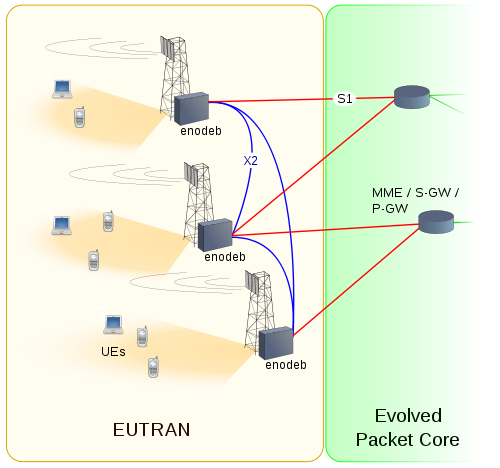
\includegraphics[scale=0.5]{EUTRAN}
\caption{Mobiiliverkon rakenne} \label{ekakuva}
\end{figure}

MEC ehdotuksia tarkasteltaessa, olemassa olevien mobiiliverkkojen arkkitehtuurit ovat keskeisessä asemassa. Useat reunalaskentaa käsittelevät ehdotukset on tarkoitettu integroitaviksi osaksi olemassa olevaa mobiiliverkkoarkkitehtuuria. 
Erityisesti asiakaslaitteiden ollessa mobiililaitteita ja mahdollisimman pieniä viiveitä tavoiteltaessa, reunalaskenta ratkaisujen integroiminen osaksi mobiiliverkkoa on väistämätöntä. Seuraavaksi käydään pääpiirteittäin läpi 4G mobiiliverkon arkkitehtuurin funktionaaliset osat.

Yksinkertaistettuna mobiiliverkko koostuu kahdesta osasta: radiorajapinnasta ja mobiilinverkon runkoverkosta (puhelinkeskuksesta?). 3GPP kehittämässä LTE standardissa radiorajapinnan sisältävä osuus on nimeltään E-UTRAN (Evolved UMTS Terrestrial Radio Access Network) ja runkoverkon osuus EPC (Evolved Packet Core).

E-UTRAN tehtävänä on toimia rajapintana asiakaslaitteen ja EPC:n välillä. Asiakaslaitteiden suuntaan yhteys on radiosignalointia ja yhtenä E-UTRAN tehtävänä onkin radioresurssien hallinointi. 
E-UTRAN sisältää verkon puolella pääasiallisena toimijana eNodeB tyyppisiä tukiasemia \cite{etsieutran}, myös muutamia poikkeustapauksia on, mutta ne jätetään käsittelemättä.
Tukiasema on asiakaslaitetta lähimpänä sijaitseva funktionaalinen verkon osa ja sen seurauksena se on houkutteleva kohde MEC ratkaisuille. Tukiasemaa voikin ajatella \textit{reunan} viimeisenä etappina ennen asiakaslaitetta. Tämä tutkielma käsittelee pääasiassa ratkaisuja, jotka keskittyvät LTE verkkoihin kohdistuvia ratkaisuja, joten tukiasemista puhuttaessa tarkoitetaan nimenomaan E-UTRAN mukaista eNodeB:tä. 

ENodeB:n tehtävänä on kommunikoida radioyhteyttä käyttäen asiakaslaitteen kanssa ja välittää molemminsuuntaista liikennettä EPC:n (Evolved packet core) suuntaan S1 rajapinnan kautta. eNodeB:t ovat myös yhteydessä toisiinsa X2 rajapintaa käyttäen. X2 rajapintaa käytetään tukiasemien väliseen kommunikointiin, joka sisältää handoverin yhteydessä tehtävää asiakaskontekstin siirtoa ja erinäisiä muita hallinnollisia toimintoja.  
Handoverin vaikutukset näkyvät myös MEC puolelle ja handoveria toimintaa käsitellään tarkemmin kappaleessa XYZ.

Mobiiliverkkojen tietoliikenne koostuu kahdesta eri tasosta: kontrollikerroksesta ja datakerroksesta.
Kontrollikerroksella on hallinnointiin liittyviä protokollia joiden tehtävänä on välittää esimerkiksi asiakaslaitteeseen liittyviä kontekstitietoja entiteetiltä toiselle. Datakerros puolestaan välittää IP liikennettä asiakkaan ja palveluiden välillä. 
EPC koostuu kolmesta alikomponentista jotka ovat MME (Mobility Management Entity), SGW (Serving Gateway) ja PGW (PDN gateway) \cite{etsilte}.
SGW:n eli palveluyhdyskäytävän tehtävänä on välittää datakerroksen liikennettä asiakaslaitteen ja ulkoisten palveluiden välillä. SGW on yhdistettynä PGW:hen, jonka tehtävänä on toimia IP tason reitittimenä EPC:n ja ulkoisen verkon välillä. PGW toimii asiakkaan ulkoverkon yhteyksien kiintopisteenä \cite{3gppepc}. MME on EPC:n hallinnollinen komponentti ja se toimii ainoastaan kontrollikerroksessa.
\subsection{Asiakaslaite}
UE (User Equipment) on yleisnimitys asiakaslaitteelle, joka hyödyntää pilven (cloud) ja reunan (edge) palveluita tietoliikenneyhteyksien avulla.
Usein käyttäjälaitteen esimerkkinä toimii jokin mobiililaite kuten puhelin, mutta myös esimerkiksi auto. 

\subsection{Edge cloud}
Edge cloud on yleisnimitys reunapalveluiden tarjoamiseen tarkoitettuille toimijoille.
Riippuen arkkitehtuurista reunapilvi koostuu yksittäisistä toimijoista tai reunaa lähellä olevista klustereista.
Edgen on mahdollista tarjota palveluita pienemmillä viiveillä ja suuremmilla tiedonsiirtokapasiteeteillä verrattuna perinteisiin pilvipalveluihin. 

\subsection{Cloud}

\subsection{Reunasolmu}
Tässä tutkielmassa reunasolmulla viitataan yksittäiseen reunalla sijaitsevaan
palvelinklusteriin, joka tuottaa asiakkaille reunapalveluita. Edge Cloud koostuu reunasolmujen joukosta.

Asiakaskohtaiselle reunainstanssille ei ole mitään vakiintunutta nimeä.
Cloudlet on yksi ehdotettu toteutustekniikka tällaiselle asiakaskohtaiselle reunalla sijaitsevalle virtuaali-instanssille \cite{satya09}.

\subsection{Software-defined networking}
Perinteinen tietoliikenneverkko koostuu joukosta erikoistuneista verkkolaitteita. 
Tällaisia laitteita ovat esimerkiksi kytkin, palomuuri ja reititin. Näiden laitteiden joukko muodostaa hajautetun rakenteen, jossa jokainen laite täytyy konfiguroida erikseen.
Laitevalmistajat tarjoavat hallinnointityökaluja, joiden avulla valmistajan omia laitteita on mahdollista konfiguroida suljettua rajapintaa käyttäen. Verkkoinfrastruktuurin hallintaa kuitenkin vaikeuttaa eri laitteiden konfiguraatioiden erilaisuus, sekä puute kokonaisvaltaiselle ohjelmalliselle konfiguroitavuudelle.
Tästä johtuen verkkoon tehtävät muutokset ovat työläitä ja riskialttiita \cite{kreutz2015software}.

Perinteisessä tietoliikennelaitteistossa tiedonvälityskerros ja kontrollikerros ovat tiukasti toisistaan riippuvaisia. Tiedonvälityskerroksella tarkoitetaan itse tietoliikennepakettien välittämiseen käytettävää kerrosta, eli tietoliikennettä ohjaavia laitteistoja. Kontrollikerroksella tarkoitetaan tietoliikenteen reitittämiseksi käytettävää logiikkaa, kuten esimerkiksi reititystauluja. Kontrollikerros on siis tällä hetkellä hajautettuna laitteiston mukana ympäri verkkoa. Tästä johtuen verkko on usein hyvin staattinen ja muutokset kankeita.

SDN (Software-defined networking) eli ohjelmallisesti määritetty verkko on yleistyvä paradigma verkkoympäristöissä.  SDN on ratkaisu, jossa tiedonvälitys- ja kontrollikerros on erotettu toisistaan. SDN:ssä ei ole erikoistunutta verkkolaitteistoa vaan nykyinen tiedonvälitykseen käytetty laitteisto korvattaisiin yleisillä reitittävillä laitteilla\footnote{Reitittämisellä tarkoitetaan tässä yhteydessä pakettien ohjausta ja välitystä yleisessä mielessä}. Kontrollikerroksen toiminnasta vastaa SDN Controller. Se on loogisesti keskitetty entiteetti, joka vastaa näiden reitittävien laitteiden ohjaamisesta.

SDN Controllerin ja reitittävän laitteiston välille oletetaan hyvin määritelty rajapinta, jonka kautta reitittäviä laitteita voidaan hallita \cite{kreutz2015software}. SDN siis toteuttaa \textit{Separation of Concerns} -periaatetta jakamalla verkon reititysmäärittelyjen konfiguroinnin ja itse laitteistopohjaisen toteutuksen omiin osiinsa. SDN Controller tarjoaa rajapinnan ylöspäin ohjelmalliselle verkkokonfiguroinnille ja hoitaa sääntöjen tulkkaamisen alaspäin. OpenFlow on yksi tunnetuimmista SDN Controllerin ja verkkolaitteiden välisestä protokollasta\footnote{\url{https://www.opennetworking.org/software-defined-standards/specifications/}}.

% TODO Flow sääntöjen toiminta.

Tarve SDN pohjaisille ratkaisuille kumpuaa jo aiemmin mainitusta konfiguraation työläydestä ja dynaamisuuden tarpeesta. Esimerkiksi virtuaalikoneiden käytön yleistyessä tarve verkon ohjelmalliselle hallittavuudelle on kasvanut \cite{jammal2014software}. Virtuaalikoneiden sijainti verkossa ei välttämättä ole kiinteä, vaan virtuaalikone saattaa siirtyä esimerkiksi migratoinnin seurauksena. Virtuaalikoneita saattaa tulla ja poistua verkosta. Perinteisessä verkkoympäristössä esimerkiksi MAC osoitetaulujen päivittäminen saattaa aiheuttaa yhteyskatkoksia palvelimeen \cite{jammal2014software}. SDN pohjaisia ratkaisuja on jo olemassa, mutta niiden käyttö ei vielä ole korvannut perinteisiä verkkolaitteita. 


\subsection{Network function virtualization} \label{nfv}
NFV (Network function virtualization) lähtee liikkeelle ongelmasta, jossa nykyisen verkkolaitteiston käyttöikä on lyhyttä ja toiminnot ovat hajautettuina useisiin suljettuihin (proprietary) laitteisiin \cite{nfvwhite}. 

NFV:n tarkoituksena on eriyttää verkkolaitteisto ja verkkotoiminnot. Tämä toteutuisi siten, että erillistä verkkolaitteistoa ei enää tarvittaisi ja nykyisten verkkolaitteiden toiminnallisuudet toteutettaisiin tavallisella palvelinlaitteistolla ohjelmatasolla. Periaate on hyvin samankaltainen kuin perinteisten palvelimien siirtyminen virtuaalikoneita hyödyntävään ympäristöön.
Virtualisoidulla verkkotoiminnallisuudella (jossain yhteyksissä VNF, Virtualized network function) tarkoitetaan ohjelmallisesti toteutettua verkkotoimintoa. Tämä mahdollistaa verkkotoiminnallisuuksien suorittamisen tavallisella palvelinlaitteistoilla hyprvisorin päällä. 

Verkkotoimintojen toteuttaminen virtuaalisina, mahdollistaisi useamman toiminnon sijoittamisen samaan laitteistoon. Tämä ainakin teoriassa mahdollistaisi myös paremman skaalautuvuuden. Myös verkkotoiminnallisuuksien käyttöönotto helpottuu mikäli erillisen laitteiston asennusta ei tarvita. Virtuaalisten verkkotoimintojen avulla on myös mahdollista säästää kaappitilaa sekä pienentää sähkönkulutusta \cite{nfvedge}.

NFV on soveltuva mille tahansa datatason (data plane) prosessoinnille ja kontrollitason (control plane) toiminnoille \cite{nfvwhite}. NFV siis soveltuu toteutustavaksi monille erilaisille verkkoitoiminnoille mobiiliverkoissa ja perinteisissä tietoliikenneverkoissa. Esimerkkeinä käyttökohteista ETSI:n NFV white paperissä on esitetty muun muassa reitittimet, palomuurit, kuormantasaajat, eNodeB:t ja MME:t. ETSI on pohtinut NFV:n laajamittaisen käyttöönoton mahdollisuuksia 5G-verkkoingrastruktuurissa ja mainitsee reunalaskennan yhtenä sen käyttötapauksena \cite{etsinfv5g}.

Yksi NFV:hen pohjautuvista ideoista on C-RAN (Cloud radio acceess network), joka pyrkii virtualisoimaan tukiaseman toinnot \cite{chih2014recent}. Käytännössä tukiaseman fyysiseen sijaintiin vietäisiin kuituyhteys ja RRU (Remote radio unit).
RRU sisältäisi radiosignalointiin tarvittavan laitteiston sekä laitteiston, joka muuttaa radion ja kuituyhteyden välillä olevaa tietoliikennettä analogisen ja digitaalisen muodon välillä.
Kuituyhteys välittää signaalin ohjelmallisesti toteutetulle BBU:lle (Baseband Unit), joka hoitaa kaikki tukiaseman toiminnot \cite{chih2014recent}.
BBU:t voitaisiin virtualisoida ja suorittaa keskitetysti palvelinsaleissa.
Toistaiseksi tukiaseman resurssit on mitoitettu suurimman mahdollisen kuorman mukaan. Virtualisoinnin avulla BBU:n resurssit olisivat paremmin skaalattavissa.
Kappaleessa \ref{concert} esitellään reuna-arkkitehtuuri, joka rakentuu C-RAN tyyliseen verkkoon.

Mobiiliverkossa toimivan reunalaskennan näkökulmasta NFV:n potentiaali on ilmeinen. Jos suurin osa mobiiliverkon toiminnoista voitaisiin virtualisoida ja siirtää tavalliselle palvelinlaitteistolle, voisi reunalaskentaa suorittaa samalla laitteistolla, eikä se vaatisi erillistä laitteistoa omille toiminnoilleen.
NFV:n haasteena on toteutuksien puute. 

\section{Ominaisuudet}

Reunalaskennan keskeisin tarkoitus on laskennan siirtäminen reunalla toimivalle reunalaskentaklusterille. Reunaa voidaan lähestyä pilven ja käyttäjälaitteiden puolelta. Käyttäjälaitteiden, kuten älypuhelimien laskentateho on suhteellisen heikkoa, lisäksi ne ovat akkuvirrasta riippuvaisia. 
Mobiililaitteen käyttöajan pidentämiseksi voidaan pyrkiä tekemään mahdollisimman vähän akkuakuluttavaa laskentaa paikallisesti, siirtämällä sitä reunalaskentaklusterille (Etsi se lähde jossa verrataan tietokoneita ja mobiililaitteita - eroa oli yhden kertaluokan verran).
Esimerkiksi verkkoliikenne mobiililaitteen ja kohdepalvelimen välillä on merkittävä viive toisi reunaklusteri palvelun huomattavasti lähemmäksi ja pienentäisi viivettä palvelussa. Viiveen pienenemisen seurauksena monet reaaliaikaisuuttaa tai nopeaa reagointia vaativat palvelut ovat mahdollisia. Lisäksi verkon viiveestä tai ruuhkasta johtuen, mobiililaitteella on usein huomattavasti nopeampi yhteys fyysisesti lähelle itseään verra

Lisäksi pilven tai konesalien suunnasta asiaa lähestyttäessä runkoverkko tukkeutuu. Siirtämällä osan palveluvastuusta reunalle, runkoverkon rasitteen tulisi ainakin periaatteessa pienentyä. 


\subsection{Etälaskenta}
Etälaskennan toteuttamiseksi tarvitaan vastaukset seuraaviin kysymyksiin. Mitä siirretään ja minne siirretään?

MOCAssa oli selitetty kuinka muodostetaan yhteys in-network cloudiin.

Etälaskenta voidaan karkeasti jakaa kahteen tyyppiin: Binääriseen ja osittaiseen \cite{mao17}. \textit{Onkohan ok lainata surveytä?}. Binäärisessä ohjelmasta suoritetaan selkeitä kokonaisuuksia joko reunasolmulla tai asiakaslaitteella. Osittaisessa etälaskennassa suoritusta siirretään dynaamisesti reunasolmulle. 

Offloading on varmaan samankaltainen termi.
Reunalla suoritettava etälaskenta saattaa siirtää ohjelman suorituksen kokonaan tai osittain asiakaslaitteelta reunasolmulle. Laskennan tulos lähetetään takaisin asiakaslaitteelle ja sitä käytetään osana muuta laskentaa. 
Laskennan hallinta suoritetaan asiakaslaitteella. Etälaskentaa motivoi raskaiden operaatioiden siirtäminen asiakaslaitteelta reunalle. Erityisesti mobiililaitteilla akkuvirran säästäminen on keskinen tekijä. Etälaskennan kannattavuus puhtaasti akkuvirran näkökulmasta muuttuu kannattavaksi, kun suoritettavan ohjelman lähettäminen ja tuloksen vastaanottaminen kuluttavat vähemmän akkua kuin ohjelman suorittaminen paikallisesti asiakaslaitteella.
Todellisuudessa pelkästään akkuvirran säästäminen ei riitä, sillä muuten laskentaa voitaisiin siirtää pilveen. QoS kuitenkin heikkenee, mikäli laskennan suorittamiseen kuluva aika pitenee huomattavasti.
Reunalle on teoriassa nopeampi yhteys ja nopeampi vastaus. Voitaisiin siis laskea että suoritusajassa mitaten ohjelman siirtäminen reunalle on kannattavaa kun suoritettavan ohjelman lähettäminen palvelimelle, sen suorittaminen ja tuloksen vastaanottaminen kestävät vähemmän aikaa kuin ohjelman suorittaminen paikallisesti. 
Ongelmana on että suorituksien aikavaatimus ei ole eksakti vaan ainoastaan arivoitavissa. Lisäksi suoritusaikainen aika-arvion tekeminen vie myös aikaa. 
Ajan ja akkuvirran säästämiseksi tehtävät toimet ovat siis keskeisimmät haasteet etälaskentaa toteutettaessa. Näiden käsittelyä ei tämän enempää tässä tutkielmassa käsitellä niiden monimutkaisuuden vuoksi.


\subsection{Etäinstanssi}
Etäinstanssissa asiakaslaitteella on yhteys reunalle. Asiakaslaitteelle tulee ainoastaan näkymä palvelun tilasta omalle laitteelleen. Vastaavasti kuin ottaisi SSH tai VNC yhteyden toiselle laitteelle. 

-Tarkista oliko jossain järkevää lähdettä tähän
\subsection{Migraatio}
Reunalaskennan migraatiolla tarkoitetaan asiakaslaitteeseen liittyvän tilan tai laskennan siirtämistä reunasolmulta toiselle.
Handoff/-over on mobiiliverkoissa yleisesti ilmenevä tilanne jossa, mobiililaitteen yhteys siirtyy tukiasemalta toiselle.
Reunalaskennassa handover tehdään reunasolmulta toiselle. Reunalaskennan
toteutustavasta riippuen, saatetaan tarvita niin sanottu live migraatio. Live migraatiossa suorituksen alla oleva sovellus tai virtuaalikone siirretään suoritusalustalta toiselle.
Tavallisesti live migraatiota käytetään palvelinkeskusympäristössä virtuuaalikoneiden siirtämiseen suorituksen aikaiseen siirtämiseen. Live migraation tavoitteena on minimoida virtuaalikoneen käyttöön kohdistuva käyttökatkon kesto.
Live migraatio toimii siten, että siirrettävää virtuaalikonetta aletaan kopioimaan kohdelaitteelle.
Koska kyseessä on suoritusaikainen kopiointi, tilan kopiointi sisältää tallennustilan ja muistin kopioinnin.
Mikäli palvelinkeskuksessa on jaettu levypalvelin, riittää ainoastaan muistin kopiointi. Tämä huomiona lähinnä siksi, että voidaan olettaa että reunasolmuilla ei ole jaettua levypalvelinta, jolloin joudutaan kopioimaan myös tallennustila. 
Kun virtuaalikoneen tila on saatu kopioitua uudelle alustalle, joudutaan kopioimaan kopioinnin aikana virtuaalikoneen tilaan tapahtuneet muutokset.
Kopiointia jatketaan iteroiden, kunnes päästään tilaan, jossa muutoksien määrä kopio-iteraatiota kohden ei enää pienene.
Tällöin alkuperäinen virtuaalikone pysäytetään ja viimeisten muutoksien kopioinnin aikana virtuaalikone ei ole käytettävissä. Tämän jälkeen migratoitu virtuaalikoneinstanssi on käytettävissä uudella alustalla. \cite{ha2015adaptive}

Reunalaskennan ja perinteisen palvelinympäristön vaatimukset live migraatiota kohtaan ovat hieman erilaiset.
Päällimmäisenä erona on migraatioon käytettävän kaistan suuruus. Palvelinsaleissa yhteysnopeudet ovat suuria ja etäisyydet verrattain lyhyitä. Lisäksi palvelinsaliympäristössä migraatioita on mahdollista tehdä koordinoidusti ilman aikarajoitteita.
Reunasolmujen välillä olevien yhteyksien nopeudet saattavat vaihdella suuresti.
Pitkä kopiointiaika johtaa pidempään käyttökatkokseen ja täten palvelun laadun heikkenemiseen. Kopiointiajan minimoimiseksi on pyrittävä pitämään siirrettävän datan määrä mahdollisimman pienenä. Reunasolmujen migraatiotarpeeseen vaikuttaa suuresti käyttäjien liikkuminen verkossa. Voidaan kuvitella tilanne jossa aamulla kaupungin keskustaan saapuvat työmatkailijat aiheuttavat "migraatiotulvan", joka ruuhkauttaa reunasolmujen käytössä olevat kaistat.  

Virtuaalikone-aihioihin perustuvassa järjestelmässä ainoastaan virtuaalikoneeseen tehdyt muutokset siirretään \cite{satya09}. Näin säästetään migraation aikana siirrettävän datan määrä.
Mikäli on tiedossa, minne käyttäjä on siirtymässä, voitaisiin migraatio tehdä suoraan kohteena olevalle reunasolmulle.
Palvelun laadun takaamiseksi migraation ennakointi on tärkeää. Mitä aikaisemmin aie siirtyä toiselle reunasolmulle tiedetään sen paremmin siihen keretään valmistautumaan. 
Migraation kesto on riippuvainen siirrettävän datan määrästä, sekä
Mikäli käyttäjä haluaa keskeyttää reunapalvelun käytön saatetaan tila tai laskenta siirtää käyttäjän laitteelle tai jättää reunalle odottamaan.

\cite{ha2015adaptive} Tukivat että migraatio virtuaalikone-aihioilla + muutoksien siirroilla aiheuttaa noin 1s downtimen hitaahkolla verkolla. Tavoitteena oli minimoida siirrettävän datan määrä ja tutkia handoff+ migraation aiheuttaman käyttökatkoksen pituutta. Testi tehtiin cloudleteillä.

MobiScudissa ja SMOREssa esitetään että käytetään livemigraatiota, mutta ei sen tarkemmin pureuduta ongelmaan. Todetaan vain että käytetään live migraatiota
\subsection{Integraatio mobiiliverkkoihin}
MEC ratkaisut ovat jakautuneet kahteen erilliseen ratkaisumalliin. 
SMOREssa ratkaisu on että SMORE nuuskii/monitoroi LTE/EPC kommunikointia ja injektoituu väliin.

\subsection{IP-verkko}
Service discovery IP-verkossa.
\subsection{Kommunikaatio asiakaslaitteen Reunasolmun kanssa}
\subsection{Hallinta}
Sisältää palveluiden etsimisen (Service Discovery) ja palveluihin ohjauksen esim Software Defined Networkingin avulla (SDN).

\section{Reunan rakenne}
Rakenteeseen vaikuttaa ehkä eniten seuraavat kaksi valintaa
\begin{itemize}
\item Kerroksittain
\item Lähelle vähän vai kauemmaksi enemmän
\end{itemize}
Molempiin ratkaisuihin liittyy omat haasteensa. Etenkin voidaan olettaa että lähelle hajalleen aiheuttaisi huomattavasti enemmän ylläpitotyötä.

\section{Esitetyt ratkaisut}
Reunalaskennasta löytyy valtavasti artikkeleita, joissa esitetään reunalaskentaan liittyvien haasteiden ratkaisuja. Ratkaisut ovat yksittäisi tapauksia eivätkä sinällään arkkitehtuuriratkaisuja. 
\subsection{Cloudlet}
Minkä ongelman cloudlet ratkaisee?
Miten cloudlet toimii?
Mitkä ovat cloudletin ongelmat?

Cloudlet on reunasolmulla suoritettava virtuaalikone-teknologiaan perustuva ratkaisu. \cite{satya09}
Virtuaalikoneisiin pohjautuva cloudlet on yksi tunnetuimmista reunapalveluiden tuottamisen konsepteista.
Cloudletin ideana on hyödyntää muokattuja virtuaalikone-instansseja, joita voidaan suorittaa reunasolmussa. 
Cloudletillä tarkoitetaan järjestelmää, joka suorittaa reunasolmulla virtuaalikoneiden hallintaan liittyviä toimia.
Yhdellä reunasolmulla voidaan siis suorittaa usean eri käyttäjän virtuaalikoneita. 

Reunan luonteesta johtuen cloudletin oletetaan ylläpitävän ainoastaan sellaisia palveluita jotka käyttävät reunaa hetkellisesti tai väliaikaisesti \cite{satya09}.
Cloudlettiä ei siis ole tarkoitettu pidempiaikaiseen tallennukseen, vaan enemminkin suoritusaikaisten tarpeiden täyttämiseen. 

Cloudletin keskeisimmäksi rakennuspalikaksi on valittu virtuaalikone. Verrattuna prosessi tai sovellus tason virtualisointiin, virtuaalikoneiden käyttö ei aseta rajoitteita palvelun toteuttamiseen käytettävään ohjelmointikieleen \cite{satya09}.
Lisäksi virtuaalikoneiden käyttö cloudlettien perustana mahdollistaa helpon tavan jakaa reunasolmun resursseja ja pitää asikaskohtaiset instanssit toisistaan erillään. 

Tavallisen virtuaalikone-kuvan suuruus tallennettuna on noin 8 gigatavua.
Koska reunasolmujen pääasiallinen idea on tarjota suoritusympäristö palveluille,
ei näin suuren tiedoston tallentaminen reunasolmulle jokaista käyttäjää kohden ole tarkoituksenmukaista.
Ja kuten jo aiemmin mainittu, reunasolmujen resurssit oletetaan rajallisiksi verrattuna palvelinsaliympäristöön.
Täten pidempiaikainen tiedostojen tallennus on parempi tehdä keskitettyihin ratkaisuihin.
Sen lisäksi että tallentaminen reunasolmuille ei ole mahdollista, kokonaisen virtuaalikoneen siirtäminen verkon yli olisi huomattavan hidasta ja se tukkisi verkon.
Siirrettävyys korostuu etenkin tilanteessa jossa siirrettäviä virtuaalikoneita olisi useita.

Cloudletin keskeisimpiä oivalluksia onkin käyttää virtuaalikoneissa yhteistä pohjaa. 
Yhteisen pohjan käyttäminen mahdollistaa sen että jokaisesta virtuaalikoneesta voidaan tallentaa vain pohjaan tehdyt muutokset.
Muutokset sisältävää tiedostoa kutsutaan pinnoitteeksi (VM overlay).
Pinnoitteen ja pohjan yhdistämiseen käytetään dynaamista virtuaalikone synteesiä.
Dynaamisuudella tarkoitetaan sitä, että käyttäjän alkaessa käyttämään cloudlet infrastruktuuri rakentaa
käyttäjän muutokset sisältävästä pinnoitteesta ja virtuaalikone-pohjasta, suoritettavan virtuaalikoneen. 
Dynaaminen virtuaalikoneiden syntetisointi edellyttää että cloudletiltä löytyy oikeanlainen virtuaalikonepohja.
Kun virtuaalikone halutaan sulkea cloudlet tallentaa virtuaalikoneeseen tehdyt muutokset pinnoitteeksi ja pakkaa tiedoston. 
Satayanaran ensimmäisessä cloudletteja käsittelevässä julkaisussa \cite{satya09} muutoksien tallentaminen pinnoitteeksi tuottaa noin 100-200 megatavun kokoisen tiedoston. Tämän kokoinen tiedosto on nykyisillä tiedosiirtonopeuksilla siirrettävissä inhimillisessä ajassa, jopa langattomien yhteyksien yli.

Cloudlettejä voi olla useita erilaisia, siispä cloudlet toiminta edellyttää että jokaisella reunasolmulla tulee olla oikean cloudlet-pohja saatavilla ja käyttäjien cloudlettien on pohjauduttava johonkin rajalliseen määrään erilaisia cloudlet pohjia.

\subsubsection*{Hallinta}

\subsubsection*{RAW – Migraatio}

Cloudlettien välinen migraatio ja handoff. 
Cloudlettien väliselle migraatiolle voi olla useita eri syitä.
Migraatio tilanteessa jossa virtuaalikone siirretään paikasta toiseen odottamaan käyttöönottoa on keskeisin.
Pelkän pinnoitteen siirtäminen riittää, mikäli tarvittava virtuaalikonepohja löytyy kohteena olevasta cloudletistä.
On kuitenkin huomattava että pinnoiteen(VM overlay) tallettamiseen voi olla kannattavaa käyttää myös asikkaan laitetta, mikäli se vain on mahdollista.
Perusteluina asiakaslaitteen käyttölle tallennusmediana voisi olla tapaus, jossa asiakas matkustaa ulkomaille ja pinnoite tulisi siirtää hyvin kaukana sijaitsevalta palvelimelta kohteena olevalle cloudletille. Tällöin saattaisi olla nopeampaa siirtää pinnoite suoraa asiakaslaitteelta.

\subsubsection*{RAW – Handoff} 


\subsection*{FMC – Follow me cloud}
\subsection{Small Cell Cloud}
Small Cell Cloud (SCC, pienisoluinen pilvi?) perusidea on reunapalveluiden integroiminen osaksi LTE-verkkoinfrastruktuuria. 
Reunaopalveluita tuotettaisiin tukiasemiin (Base Station) sijoitetuilla palvelinresursseilla.
LTE mahdollistaa heterogeenisten verkkojen luomisen. Matkapuhelinverkkojen tapauksessa tällä tarkoitetaan sitä, että yksittäisen solun sisällä saattaa olla pienempiä soluja.
Verkko saattaa siis koostua useammasta kerroksesta erikokoisia soluja. 
Kun solut ovat muuttumassa pienemmiksi tukiasemat tulevat fyysisesti lähemmäksi käyttäjää.

SCC tarkoituksena on hyödyntää solujen pienentymistä, tuomalla niihin reunapalveluiden tuottamisen mahdollistavaa teknologiaa.
SCC reunalaskentapalvelut tuotetaan SCeNBce klustereissa. 
SCeNBce (Small-cell eNodeB computing-enhanced) on palvelinresursseilla varustettu eNodeB tukiasema \cite{lobillo15scc}.
Verrattuna cloudletteihin, SCeNBce:ssä palvelinresurssit ovat tiiviisti osana tukiasemaa.

SCM (Small Cell Manager) on SCC arkkitehtuurissa hallinnasta vastaava komponentti. Normaalisti LTE verkossa keskeinen hallinnosta vastaava komponentti on Mobility Management Entity (MME). Sen tehtäviin kuuluu on hoitaa muunmuassa MME:ltä toiselle tapahtuvat handoverit ja asiakkaiden autentikointi. Täten on luonnollista että SCM liitetään MME:n yhteyteen, jossei suorasti niin ainakin jonkin yhteyden välityksellä. Eräs ehdotettu tapa toteuttaa SCM onkin integroida se suoraan MME:n yhteyteen jolloin tämä komponentti vastaa sekä reunapalveluista ja LTE-verkon hallinnasta\cite{lobillo15scc}. SCM tehtävänä on organisoida resurssien utilisointia SCeNBce klustetereiden välillä. Tähän kuuluu esimerkiksi palvelinresurssien sammuttaminen mikäli ne eivät ole käytössä ja mahdollisesti yliutilisoidulta SCeNBce:ltä kuorman siirtäminen toiselle SCeNBce:lle. Tämän lisäksi esimerkiksi virtuaalikoneiden migraatiopäätöksien tekeminen on SCM tehtävä.

Koska SCC:n tapauksessa palveluiden tuottamiseen käytettäisiin matkapuhelinverkkoa, rajaisi se myös asiakaslaitteet älypuhelimiin ja muihin tätä verkkoa käyttäviin laitteisiin.
Reunapalveluiden sitominen tiukasti matkapuhelinverkkoon vaikuttaa erikoiselta.
Ratkaisulla on hyvät ja huonot puolensa. Reunapalveluiden tarjoamisen muihin verkkoihin, esimerkiksi WiFi yhteydellä ei onnistu suoraan ehdotetulla 

SCC:n arkkitehtuurin haasteena saattaa olla niiden ylläpidettävyys, jossa matkapuhelinverkko-operaattori on vastuussa reunasolmun ylläpidosta, koska se on tiukasti sidoksissa tukiasemaan\cite{lobillo15scc}.
Tukiasemaan tiukasti sidotulla ratkaisulla on kuitenkin mahdollista hyödyntää laajemmin tukiaseman ominaisuuksia, kuten radioyhteyksiä toisiin tukiasemiin.
SCeNBce tukiasemien hankkiminen vaatii operaattoreilta investointeja sekä lisää ylläpitotyön määrää. (Näiden vuoksi ehkä kantsis miettii, että miksi se on niin tiukasti kiinni siinä televerkossa. Muutenkin useampi operaattori samalla alueella tarkoittaa että jokaisella on myös omat reunapalvelut, joka taas meinaa kokonaiskuvassa että sama palvelu pitää duplikoida monelle operaattorille.)

\subsubsection{Kommunikointi reunapalveluun}
SCC pohjaisessa järjestelmässä tavallinen verkkoon menevä tietoliikenne ja reunapalvelulle menevä tietoliikenne on ehdotettu eroteltavaksi toisistaan \cite{puente15seamless}.
Eristyksen seurauksena LTE-A arkkitehtuuriin ei tarvitse koskea muutoin kuin lisäyksien osalta. 
Liikenne SCeNBce:llä tarjottuihin reunapalveluihin on tehtävä tarkoitusta varten olevan rajapinnan kautta.
Asiakaslaitteelta tuleva liikenne reititetään SCeNBce:llä. 
Pakettien reitittämiseksi SCeNBce joutuu päättelemään, onko paketin määränpää reunapalvelu vai tavallinen tietoliikenne.

 Koska LTE-tukiasemat eivät toimi IP tasolla, ei reunapalvelulta tuleva pakettiliikenteen sisältämä asiakaslaitteen IP-osoite riitä identifioimaan kohdelaitetta. 
Yleisesti LTE verkossa, internetistä asiakaslaitteelle suuntautuvan liikenteen osalta pakettien ohjaamiseksi, käytetään GTP-tunnelia. GTP-tunnelilla tietoliikenne saadaan ohjattua oikealle tukiasemalle.
Tukiaseman ja asiakaslaitteen välisen kommunkaatioväylän selvittämiseksi joudutaan tekemään TEID (Tunnel endpoint IDentifier) ja DRB-ID (Data Radio Bearer ID) muunnos.

Vastaava ongelma on myös reunapalvelulta asiakaslaitteelle suuntautuvassa tietoliikenteessä.
SCC:n yhteydessä ehdotetussa ratkaisussa reunapalvelulta tulevan liikenteen yhdistäminen asiakaslaitteen IP-osoitteeseen voidaan tehdä käyttäen TEID perustuvaa ohjaustaulua.
TEID on asiakaskohtaisen GTP-tunnelin indetifioiva tunniste.
TEID:stä ja asiakaslaitekohtaisesta IP-osoitteesta voidaan muodostaa SCeNBce:lle reititystaulu. 
Reititystaulun avulla voidaan ohjata IP-osoitte muuntaa DRB liikkenneväyläksi ja ohjata tietoliikenne asiakaslaitteeseen.

 
\subsection{SMORE ja MobiScud}
SMORE (Software defined network Mobile Offloading aRchitecturE) on toinen televerkkoihin suunniteltu MEC ratkaisu. \cite{cho2014smore}
SMORE:n keskeisin sisältö on ottaa SDN (Software Defined Networking) käyttöön reunapalveluiden saavuttamiseksi. SDN käyttöönotolla tavoitellaan sitä, että televerkon toimintaan ei tarvitsisi tehdä muutoksia. Minkään olemassa olevan komponentin toiminta ei siis muutu. 
SMORE:n toiminta on jaettu kahteen osaa, joita varten SDN on käytössä. 
Ensimmäisenä on mobiiliverkon kontrollitasolla (control-plane) tapahtuva viestien monitorointi. 
Toisena toimintona on monitoroitujen tietojen pohjalta tehtävät SDN hallintatoimenpiteet. Näiden avulla voidaan ohjata haluttu osa tietoliikenteestä haluttuihin reunalaskentayksikköihin.
Kontrollitasolla viestejä monitorointia suorittaa SMORE monitori (SMORE monitor) ja tietoliikenteen ohjauspäätöksistä vastaava komponentti on SMORE kontrolleri (SMORE controller).

Tietojen välitys SMORE kontrollerin ja SMORE monitorin välillä on toteutettu yhteisen tietokannan kautta. SMORE monitor tallentaa poimitut tiedot tietokantaan ja antaa tiettyjen tapahtumien yhteydessä SMORE kontrollerille herätteen tehdä asianmukaiset muutokset SMORE:n SDN reitityksiin. Herätteitä laukaisevat tapahtumat ovat asikkaan liittyminen verkkoon ja asikkaan liikkuminen verkossa.

SMORE monitori tarkkailee asiakaslaitteen ja LTE/EPC:n välistä liikennettä.
Asiakaslaitteen liittyessä mobiiliverkkoon, asiakaslaite ja LTE/EPC:n sisäiset komponenti muodostavat tunneleita ja asiakaslaitteeseen liitetään erilaisia tunneleita koskevia osoite ja metatietoja.
SMORE monitorin tehtävänä on poimia asiakaslaitteen liittyessä ja yhteydenmuodostuksen aikana asiakaslaitteisiin liittyviä tietoja.
Asiakaslaitteen lähettäessä liittymispyynnön (attach request) SMORE monitori poimii pyynnöstä asiakaslaitteen IMSI (international Mobile Subscriber Identity) ja TAI:n (Tracking Area Identifier). 
Tämän jälkeen SMORE monitori poimii MME:n asiakaslaitteelle lähettämästä liittymispyynnön hyväksymis -viestistä (attach accept) monitori poimii asiakaslaitteelle annetun IP-osoitteen, SGW:n IP-osoitteen, SGW:n TEID:n ja asiakaslaitteen GUTI:n (Globally Unique Temporary Id).
Tämän jälkeen eNodeB neuvottelee asiakaslaitteen kanssa radioyhteydestä ja tämän lopputulos välitetään MME:lle. SMORE monitor poimii eNodeB:n ja MME:n välisestä kommunikaatiosta eNodeB:n IP-osoitteen ja eNodeB:n TEID:n.
Kun edellä mainitut tiedot on tallennettu SMORE:n tietokantaan, SMORE monitor lähettää SMORE kontrollerille herätteen päivittää SDN reitityksiä. 

Toinen tapahtuma josta SMORE kontrolleri on kiinnostunut on handover, eli mikäli asiakaslaite siirtyy mobiiliverkossa eNodeB:den välillä. SMORE kontrollerin on tässä tapauksessa kiinnostunut mobiiliverkossa tapahtuvista muutoksista. 
Handover alkaa kun tällä hetkellä käytössä oleva eNodeB päättää, että on aika siirtää asiakaslaitteen yhteys toiselle eNodeB:lle (kohde).
Alkuperäinen eNodeB välittää pyynnön kohteena olevalle eNodeB:lle joka oletettavasti hyväksyy sen. Tämän jälkeen, kohteena oleva eNodeB pyytää MME:ltä reitityksen muutosta. Tässä välissä oleva SMORE monitor poimii reitityksen muutosta koskevan tiedon ja välittää ne SMORE kontrollerille.
Tämän tiedon pohjalta SMORE kontroller voi tehdä SDN muutokset siten että vanhat reititykset voidaan poistaa ja korvata uusilla.


\subsubsection{MobiScud}
MobiScud \cite{wang2015mobiscud} on SMORE:n ideoita ammentava versio reunalaskentapalveluiden tuottamisesta mobiiliverkoissa.
MobiScud:in perustoiminnallisuus on hyvin samankaltainen kuin SMORE:ssa. MobiScud painottaa enemmän käyttäjän tarvetta liikkua verkossa. Lisäksi MobiScud käyttää hyödykseen oletusta mobiiliverkkojen hajautettua rakennetta. 

Kuten SMORE, MobiScud käyttää hyödykseen SDN:n tarjoamia ominaisuuksia ja siten olettaa sen käyttöönottoa palveluntarjoajan infrastruktuurissa. Lisäksi MobiScudin toiminnallisuudet on ajateltu toteutettavan Network Function Virtualisantionin (NFV) avulla. 
MobiScud Controller (MC) koostuu kahdesta loogisesta kokonaisuudesta: monitorista ja kontrollerista. Näiden toimintaperiaate on käytännössä identtinen SMORE:n vastaavan nimisiin toimijoihin. MC:n sijaintia ei kuitenkaan ole keskitetty kuten SMORE:ssa vaan sen oletetaan sijaitsevan hajautettna RAN ja EPC välissä.
Käyttäjän ja reuna-infrastruktuurin välinen yhteys toteutetaan hyvin samalla tavalla kuin SMORE:ssa. 

MobiScudin reunapalvelut on ajateltu toteutettavan hyvin cloudletmäisesti. Mahdollisimman lähellä reunaa sijaitsevassa "pilvessä" on palvelinresursseja, joita käyttäjät hyödyntävät yksityisien virtuaalikoneinstanssien muodossa (Private Virtual Machinem, PVM). 

MobiScudin tavoitteena on tarjota asiakkaalle mahdollisimman nopea yhteys asiakkaan ja PVM:n välille. MobiScud hyödyntää televerkon omia kontrollitason viestejä asiakkaan liikkumisen seuraamiseen. Kun handoverista tulee viesti MC:n monitoroivalle entiteetille, alkaa MC organisoimaan reunalaskentaan liittyviä muutoksia. 

Asiakkaan siirtyessä tukiasemalta toiselle PVM:n siirto aloitetaan livemigraationa kohteena olevalle "pilvelle". Livemigraation ollessa käynnissä kohteena olevan pilven MC huolehtii että asiakaslaitteella on edelleen yhteys alkuperäiseen sijaintiinsa. Tämä hoidentaan SDN reititysmuutoksilla. Kun PVM:n livemigraatio on saatu suoritettua alkuperäisen sijainnin MC ilmoittaa tästä kohdesijainnin MC:lle, joka puolestaa päivittää SDN reititykset ohjaamaan siirretylle PVM:lle.

MobiScudin testeissä livemigraation ja SDN reitityksien avulla RTT (round trip time) saatiin pidettyä pienenä. Kuitenkin yhteyksissä aiheutui noin kahden sekunnin mittaisia katkoksia sillä hetkellä kun livemigraation viimeiset muutokset lähetetään. Yhteyskatkoksen pituuteen vaikuttavat monet asiat ja artikkelissa huomautetaankin että nykyinen toteutus oli optimoimaton ja vaatii jatkotutkimuksia.


\subsection{Concert}
Nykyinen LTE televerkko koostuu joukosta laitteita, joilla on hyvin spesifit tehtävät. CONCERT pyrkii seuraavan sukupolven televerkkoihin keskittyvässä ratkaisussaan vähentämään tehtäväspesifien laitteiden tarvetta. 
CONCERT arkkitehtuuri koskee siis pääasiassa seuraavan sukupolven televerkkoja, vaikkakin sen ratkaisut mahdollistavat tuen myös vanhemmille teknologioille. CONCERT esittää uudenlaista toiminnallisuuksien toteuttamismallia, joka korvaisi valmistajakohtaisia telelaitteita (kuten tukiasemat) virtualisoiduilla ja ohjelmistopohjaisilla ratkaisuilla. NFV ja SDN käyttöönotto toimii siis tämänkin ehdotuksen selkärankana.
Verkon toimintojen virtualisointi mahdollistaa laitteiston siirtämisen kauemmaksi reunasta, joka osaltaan vähentää hajautettavan laitteiston määrää. CONCERTin ideana on, että hajautetuksi jäisi telelaitteistosta ainoastaan välttämättömin osa, eli radiorajapinnan mahdollistava RIE (Radio Interfacing Equipment) ja hierarkisesti jaetut reunalaskentayksiköt. Televerkon muita toiminnallisuuksia voitaisiin keskittää ja tarjota virtuaalisina ohjelmistoteutuksina. 

Conductor on CONCERT arkkitehtuurissa hallinnollisessa keskiössä ja se vastaa päällysverkon hallinnasta.
CONCERT arkkitehtuurissa control ja data planet on erotettu toisistaan ja Conductorin tehtävänä esittää data planella esiintyvät fyysiset resurssit virtuaalisina resursseina.
Reunalaskentayksiköiden resurssien jakaminen sekä niiden välisten SDN kytkimien kautta muodostettujen yhteyksien hoitamisesta vastaa conductor.
Conductorin toiminta on toistaiseksi kuvattu vain korkealla tasolla, joten sen toteutustekniset ratkaisut ovat avoimia.

Vaikka laitteiston virtualisointi ja palveluiden keskittäminen kustannuksien säästämiseksi kuulostaakin houkuttelevalta, on kesittämisessä myös omat ongelmansa.
Etenkin liiallinen keskittäminen siirtää verkon toiminnallisuuksia kauemmaksi reunasta, joka osaltaa johtaa korkeampiin latensseihin ja heikentää palvelun laatua. Vaikka conductor onkin esitetty yksittäisenä loogisena entiteettinä, sen toiminnallisuuksia on mahdollista porrastaa ja hajauttaa paremman skaalautuvuuden ja pienempien latenssien tavoittamiseksi.

CONCERTin ratkaisu reunapalveluiden tuottamiseksi on hierarkinen kolmeen tasoon jaettu arkkitehtuuri.
\textit{Paikalliset} reunalaskentaresurssit sijaitsevat kaikkein lähimpänä verkon reunaa, esimerkiksi RIE:n kanssa samassa sijainnissa sijaitseva palvelin. Paikallisen reunalaskentayksikön laskentaresurssit ovat rajalliset ja sen tehtävänä onkin suorittaa ainoastaan kaikkein tiukimman aikavaatimuksen laskentaa.
\textit{Alueelliset} reunalaskentaresurssit kattavat jonkin pienen alueen reunalaskenta tarpeita ja korkeimman tason \textit{keskus} reunalaskentaresurssit kattavat jonkin suuremman alueen resurssi intensiivistä reunalaskentaa.
CONCERT:ssa reunalaskentaresurssien jakamisesta vastaa conductorin sisäinen komponentti LCM (Location-aware computing management).


 Reunalaskennan osalta CONCERTissa resurssit on jaettu hierarkisesti kolmeen tasoon, siten että lähimpänä käyttäjää on \textit{paikalliset} palvelimet, jotka on tarkoitettu kaikkein tiukimman aikavaatimuksen sovelluksille. Seuraavat kaksi tasoa, \textit{alueellinen} ja \textit{keskus (central)}, kasvattavat palvelinresurssien määrää, mutta ovat kauempana reunasta. Reunalaskentayksiköt voivat olla yhteydessä toisiinsa, jolloin ne mahdollistavat nopeat M2M (Machine-to-Mahcine) yhteydet. Tämä mahdollistaisi muunmuassa autojen välisen kommunikaation reunaverkon välityksellä. 

Toistaiseksi CONCERT on korkean tason suunnitelma ja se käyttää hyväkseen vielä olemassa olemattomia teknologisia ratkaisuja kuten tukiasemien virtualisointia. Arkkitehtuuri mahdollistaa erilaisien ratkaisujen toteuttamisen, eikä aseta tiukkoja rajoitteita resurssien tai hallinnon sijoittelun suhteen.

\subsection{ETSI MEC}
\subsection{ETSI MEC}
ETSI (European Telecommunications Standards Institute) on eurooppalainen telealan standardointijärjestö.
ETSI on aloittanut reunalaskennan arkkitehtuurin, sekä sen touteuttamiseksi vaadittavien toimintojen standardoimisen.

ETSIn MEC spesifikaatio määrittelee reunapalvelun tuottamiseksi vaadittavat ominaisuudet, jotka reunainfrastruktuurin tulee toteuttaa.
Spesifikaatio listaa myös mahdollisia, mutta ei vaadittuja toimintoja. 
Listaamalla vaaditut toiminnot stanrardi pyrkii yhtenäistämään reunalaskennan konsepteja.  

\subsubsection{Vaatimukset}
Vaatimukset on jaettu kategorioihin sen mukaan mihin toiminnallisuuteen vaatimus liittyy.
Vaatimuksien kategoriat ovat yleiset vaatimukset (generic requirements), palvelu vaatimukset (service requirements), hallinta vaatimukset (operation and management requirements) ja viimeisenä kategoriana on kokoelma vaatimuksista, joiden teemoina ovat turvallisuus, sääntely ja veloitus (Security, regulation, charging requirements)\cite{etsitechreq}. 

Yleiset vaatimukset ovat luonteelta korkean tason kuvauksia reuna-infrastruktuurin toiminnallisuuksista. Yleiset vaatimukset kategorisoitu seuraaviin luokkiin: viitemallista, reunapalvelun sovelluksien elinkaaresta (application lifecycle),
reunapalvelun sovellusympäristöstä (application enviroment) sekä liikkuvuuden tuesta (support of mobility).
Viitemallin tulee vaatimuksien mukaan hyödyntää mukaan NFV ratkaisuja hallinnollisten toimien toteuttamiseen, mikäli mahdollista. 
ETSI:n vaatimuksen mukaan reunapalvelun tulee voida sijaita käytännössä missä tahansa kohdassa radiomaston runkoverkon reunan välillä. Sijainnin vapaus myös tarkoittaa että reuna-alusta(?) ei voi olla riippuvainen alla olevasta infrastruktuurista. 
Reunapalvelun sovelluksien elinkaareen liittyvät vaatimukset koskevat pääasiassa reunapalvelun toimijoiden oikeuksia päättää reunan sovelluksien käynnistämisestä ja sulkemista.
Reunapalveluiden sovellusympäristöä koskevissa vaatimuksissa esitetään, että sovelluksien autenttisuus ja eheys pitää pystyä varmentamaan. Sovellusympäristön täytyy myös mahdollistaa reunasovelluksen käyttöönotto toisella reuna-isännällä, ilman erikoisempaa mukautusta (without specific adaptation) \cite{etsitechreq}.
Mobiiliverkkojen ollessa kyseessä, asiakaslaitteiden liikkuminen tukiasemalta toiselle, on keskeinen käyttötapaus. Tämä heijastuu myös vaatimukseen liikkuvuuden tukemisesta reunapalveluissa.
Vaatimuksena on että asiakaslaitteen ja reunapalvelun välisen yhteyden tulee säilyä, vaikka asiakaslaite siirtyisi solusta toiseen tai asiakaslaite siirtyisi sellaiseen soluun joka on toisen reuna-isännän vastuualuetta.

Palveluvaatimukset on joukko vaatimuksia, jotka keskittyvät takaamaan reuna-infrastruktuurin perimmäiset palveluperiaatteet.
Lista palveluvaatimuksista on pitkä, joten tähän tutkielmaan on poimittu ainoastaan osa vaatimuksista. Täydellinen lista löytyy \cite{etsitechreq} julkaisusta.
Palveluvaatimukset kuvaavat toiminnallisuuksia, joiden avulla reunapalveluita voidaan tuottaa. Tällaisesta esimerkkinä tietoliikenteen reitittämiseen liittyvät vaatimukset, joiden keskeinen tehtävä on kuvata mahdolliset tietoliikennereitit reunapalveluun ja ulos reunapalvelusta. Yksi ehkä keskisimmistä palveluvaatimuksista on reuna-alusta mahdollisuus suodattaa ja muokata verkkoliikennettä. 
Lisäksi kuvataan että reunapalveluiden toimintaa ei haluta rajoittaa pelkästään asiakas-palvelu tyyppisen toimintamalliin. Reunapalveluiden tuottamiselle onkin annettu mikropalvelu -tyyppinen (microservice) kuvaus, jossa palveluntuottajat voivat toimia myös toisten reunapalveluiden kuluttajana (consumer).

\subsubsection{Viitekehys ja referenssiarkkitehtuuri}

ETSIn esittämän viitekehys esittää reunalaskentaan liittyvät korkean tason entiteetit. Nämä entiteetit on jaettu kolmeen tasoon: järjestelmä, isäntä ja verkko(system, host ja network). 
Verkkokerros sisältää verkkoyhteyksistä vastaavat entiteetit. MEC:n tapauksessa verkkokerros koostuu ainakin kolmesta osasta: sisäverkko, ulkoverkko ja televerkko.
Isäntäkerros koostuu reunapalveluiden virtualisointiin ja reunapalvelun hallinointiin keskittyvistä entiteeteistä.
Järjestelmäkerros koostuu korkeamman tason hallinnosta vastaavista elementeistä.

Referenssiarkkitehtuurissa on esitetty funktionaaliset entiteetit. Funktionaalisten entiteettien toiminta on kuvattu 
Referenssiarkkitehtuurissa reuna-isännällä (edge-host) tarkoitetaan entiteettiä, joka tarjoaa virtualisointi-infrastruktuurin, sekä reunalaskennan toteuttamiseen vaadittavat resurssit (laskenta, tallennus ja verkko).
Reuna-alustalla (Mobile edge platform) tarkoiteen sitä entiteettiä joka mahdollistaa reunapalveluiden käyttämisen. Reuna-alusta siis mahdollistaa reunapalveluiden saavuttamisen, eli käytännössä tarjoaa rajapinnan asiakaslaitteen suuntaan. Tähän kuuluu siis palvelurekisterin ylläpitäminen, reitityssääntöjen ylläpitäminen, sekä liikenteen välittäminen reunapalveluille. Reuna-alusta voi myös itse tarjota  palveluita.
Esimerkkinä tällaisesta voisi olla tunnistautumispalvelu. 
Reuna-applikaatioilla tarkoitetaan reuna-alustalla suoritettavia virtuaalikoneita, jotka suorittavat reunapalveluiden tuottamiseksi tarkoitettuja ohjelmistoja.


\subsection{Yhteenveto}

 
\bibliographystyle{apalike}

\bibliography{lahteet}

\lastpage

% --- Appendices ---

% uncomment the following

% \newpage
% \appendix
% 
% \section{Esimerkkiliite}

\end{document}
